\documentclass[12pt]{article}
\usepackage{tikz}
\usepackage{pdflscape}


\pagestyle{empty}
\begin{document}
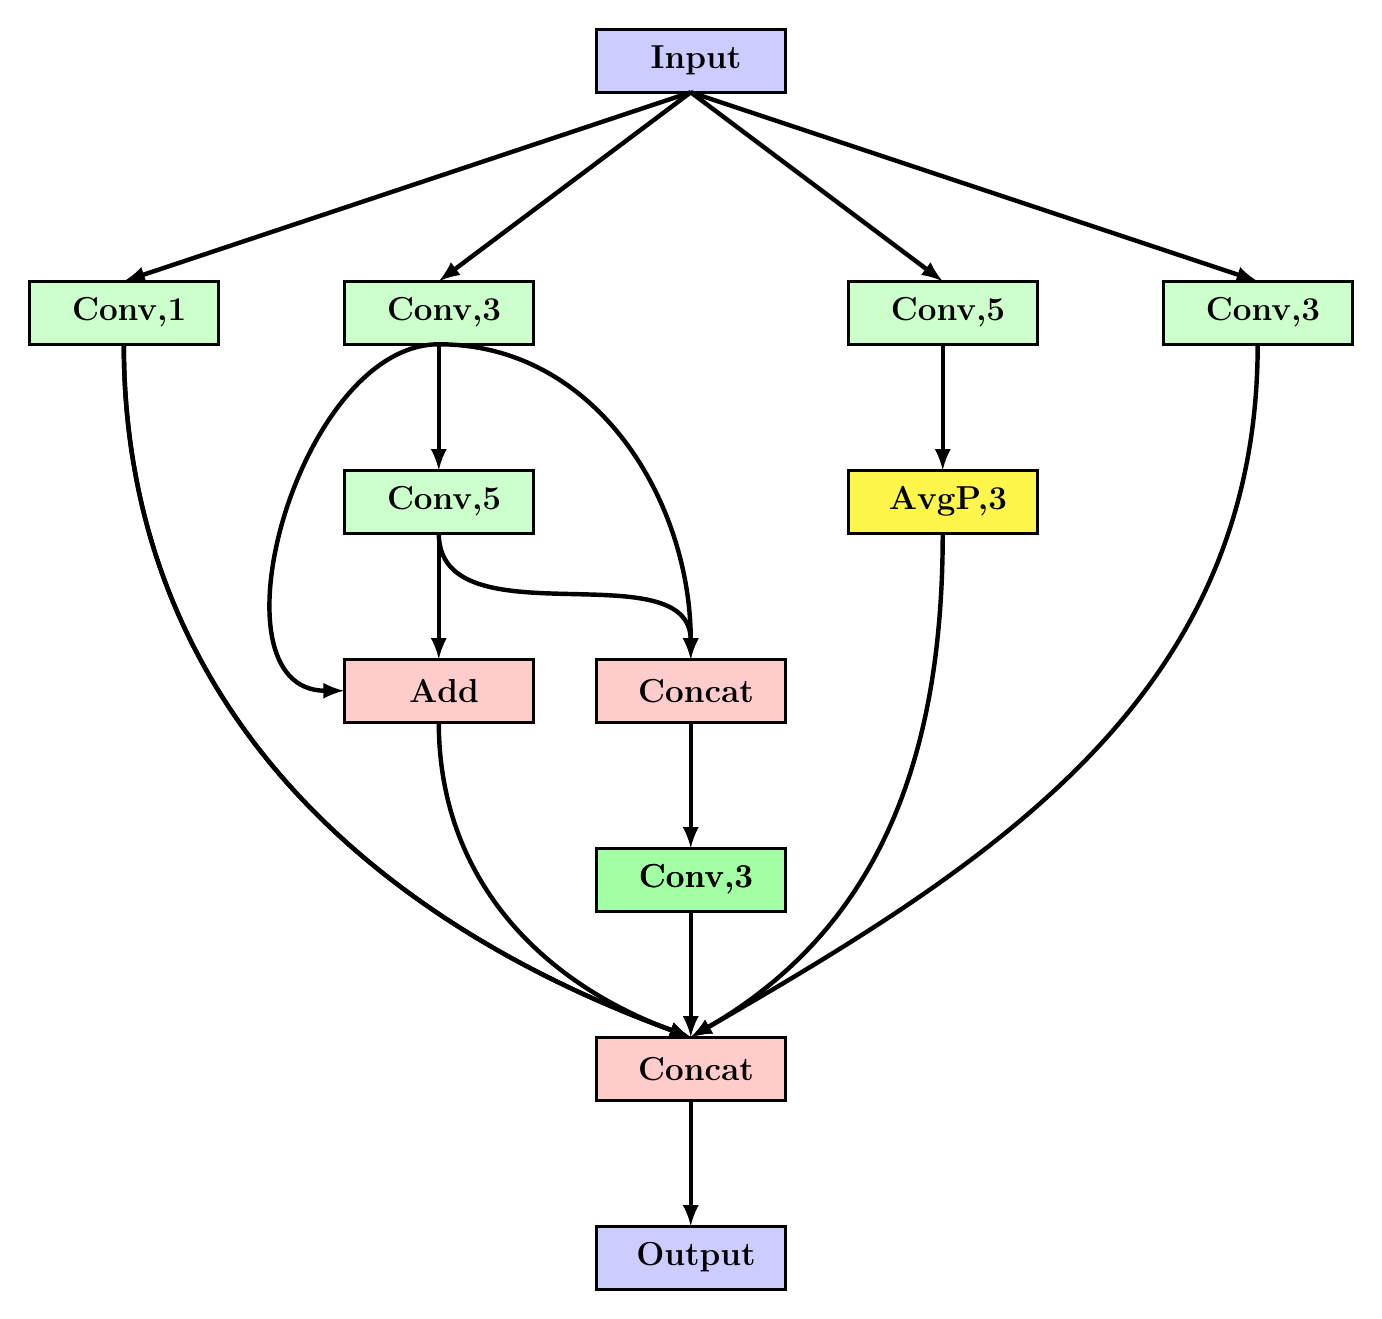
\begin{tikzpicture}[scale=0.8]
\centering
% Input
\fill[blue,fill opacity=0.2] (11,20) rectangle (14,21);
\draw (12.5,20.5) node {\textbf{ \large Input}} ;
\draw[black,very thick](11,20) rectangle (14,21);


%Conv,1
\fill[green,fill opacity=0.2] (2,16) rectangle (5,17);
\draw (3.5,16.5) node {\textbf{ \large Conv,1}} ;
\draw[black,very thick](2,16) rectangle (5,17);

%Conv,3
\fill[green,fill opacity=0.2] (7,16) rectangle (10,17);
\draw (8.5,16.5) node {\textbf{ \large Conv,3}} ;
\draw[black,very thick](7,16) rectangle (10,17);
%Conv,3 %Conv,5
\fill[green,fill opacity=0.2] (7,13) rectangle (10,14);
\draw (8.5,13.5) node {\textbf{ \large Conv,5}} ;
\draw[black,very thick](7,13) rectangle (10,14);
%Conv,3 %Conv,5 %Add
\fill[red,fill opacity=0.2] (7,10) rectangle (10,11);
\draw (8.5,10.5) node {\textbf{ \large Add}} ;
\draw[black,very thick](7,10) rectangle (10,11);
%Conv,3 %Conv,5 %Add %Concat
\fill[red,fill opacity=0.2] (11,10) rectangle (14,11);
\draw (12.5,10.5) node {\textbf{ \large Concat}} ;
\draw[black,very thick](11,10) rectangle (14,11);
%Conv,3 %Conv,5 %Add %Concat % Conv,3
\fill[green,fill opacity=0.2] (11,7) rectangle (14,8);
\draw (12.5,7.5) node {\textbf{ \large Conv,3}} ;
\draw[black,very thick](11,7) rectangle (14,8);

%Conv,3 %Conv,5 %Add %Concat % Conv,3
\fill[green,fill opacity=0.2] (11,7) rectangle (14,8);
\draw (12.5,7.5) node {\textbf{ \large Conv,3}} ;
\draw[black,very thick](11,7) rectangle (14,8);



%Conv,5
\fill[green,fill opacity=0.2] (15,16) rectangle (18,17);
\draw (16.5,16.5) node {\textbf{ \large Conv,5}} ;
\draw[black,very thick](15,16) rectangle (18,17);

\fill[yellow,fill opacity=0.7] (15,13) rectangle (18,14);
\draw (16.5,13.5) node {\textbf{ \large AvgP,3}} ;
\draw[black,very thick](15,13) rectangle (18,14);

%Conv,3
\fill[green,fill opacity=0.2] (20,16) rectangle (23,17);
\draw (21.5,16.5) node {\textbf{ \large Conv,3}} ;
\draw[black,very thick](20,16) rectangle (23,17);


%Concat
\fill[red,fill opacity=0.2] (11,4) rectangle (14,5);
\draw (12.5,4.5) node {\textbf{ \large Concat}} ;
\draw[black,very thick](11,4) rectangle (14,5);

%Output
\fill[blue,fill opacity=0.2] (11,1) rectangle (14,2);
\draw (12.5,1.5) node {\textbf{ \large Output}} ;
\draw[black,very thick](11,1) rectangle (14,2);

\draw[-latex,ultra thick, black] (12.5,20)to(3.5,17); 
\draw[-latex,ultra thick, black] (12.5,20)to(8.5,17); 
\draw[-latex,ultra thick, black] (12.5,20)to(16.5,17); 
\draw[-latex,ultra thick, black] (12.5,20)to(21.5,17); 


\draw[-latex,ultra thick, black] (8.5,16)to(8.5,14); 
\draw[-latex,ultra thick, black] (8.5,13)to(8.5,11); 

\draw[-latex,ultra thick, black] (12.5,10)to(12.5,8); 
\draw[-latex,ultra thick, black] (12.5,7)to(12.5,5);
 
\draw[-latex,ultra thick, black] (16.5,16)to(16.5,14); 

\draw[-latex,ultra thick, black] (12.5,4)to(12.5,2); 

 
\draw[-latex,ultra thick, black] (8.5,16)to[out=180,in=180] (7,10.5); 
\draw[-latex,ultra thick, black] (8.5,16)to[out=0,in=90] (12.5,11); 
\draw[-latex,ultra thick, black] (8.5,13)to[out=270,in=90] (12.5,11); 

\draw[-latex,ultra thick, black] (8.5,10)to[out=270,in=160] (12.5,5); 
\draw[-latex,ultra thick, black] (3.5,16)to[out=270,in=160] (12.5,5); 

\draw[-latex,ultra thick, black] (3.5,16)to[out=270,in=160] (12.5,5); 

\draw[-latex,ultra thick, black] (16.5,13)to[out=270,in=30] (12.5,5); 
\draw[-latex,ultra thick, black] (21.5,16)to[out=270,in=30] (12.5,5); 


\end{tikzpicture}

\end{document} 